\chapter{Rust}

\section{安装和配置}
默认情况下,Rust及其工具集Cargo都会被安装到/root/.rust和/root/.cargo,或者
是C:$\backslash\backslash$Users$\backslash\backslash$zhangjl$\backslash\backslash$AppData下,
只针对当前用户有效。有的时候,我们需要针对所有用户有效,因此,需要更改安装
路径。Rust提供了2个环境变量,进行安装路径的修改,其使用如下:
\begin{code-block}{bash}
export CARGO_HOME=/opt/cargo
export RUSTUP_HOME=/opt/rustup
export PATH=/opt/cargo/bin:$PATH
\end{code-block}

Windows,则是修改系统的环境变量,将CARGO\_HOME和RUSTUP\_HOME指向合适的
位置即可。然后再执行安装程序即可(windows执行可执行程序):
\begin{code-block}{bash}
curl --proto '=https' --tlsv1.2 -sSf https://sh.rustup.rs | sh
\end{code-block}

安装完毕之后,通常需要进行一些安装和配置,方便其他的代码编辑器可以使用代码
补全。操作如下(Linux/Windows通用):
\begin{code-block}{bash}
rustup toolchain add nightly
rustup component add rust-src rls rust-analysis
cargo +nightly install racer
\end{code-block}

如果需要对Rust和相关的工具进行升级,则操作如下:
\begin{code-block}{bash}
rustup update
cargo +nightly install racer
\end{code-block}

\section{Rust的交叉编译}
Rust本身也支持进行交叉编译,可以在Linux下完成针对ARM/Windows的目标文件的编译。
默认情况下,Rust的工具链只会包含当前操作系统默认支持的工具链。查看工具链可
如下操作:
\begin{code-block}{bash}
rustup target list
\end{code-block}

其结果大致如下图\nameref{fig:rust_target}所示。
\begin{figure}[H]
  \centering
  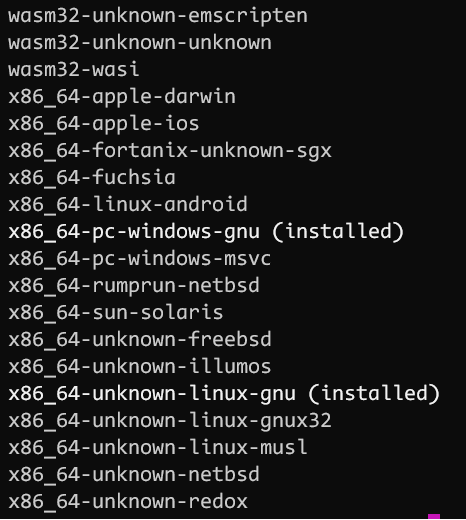
\includegraphics[scale=0.5]{rust_target.png}
  \caption{Rust支持的目标文件架构}
  \label{fig:rust_target}
\end{figure}

需要编译对应架构的目标文件,则需要添加对应架构的工具链
\begin{code-block}{bash}
# 针对ARM V7架构的工具链
rustup target add armv7-unknown-linux-gnueabihf
# 针对ARM X64架构的工具链
rustup target add aarch64-unknown-linux-gnu
# 针对Windows 64的工具链
rustup target add x86_64-pc-windows-gnu
\end{code-block}

除了添加工具链之外,还需要安装对应的交叉编译工具
\begin{code-block}{bash}
# 针对Windows 64的交叉编译工具
dnf install mingw64-gcc mingw64-winpthreads-static -y
\end{code-block}

而针对ARM V7以及ARM X64的交叉编译工具,则是使用gcc-linaro工具链即可。

针对Windows 64的交叉编译方法比较简单,其编译指令如下:
\begin{code-block}{bash}
cargo build --release --target=x86_64-pc-windows-gnu
\end{code-block}

针对ARM V7和ARM X64的编译过程稍微复杂一些,其操作如下:
\begin{enumerate}
  \item 创建配置文件:进入rust工程的根目录
\begin{mdframed}[topline=false, bottomline=false, leftline=false,
    rightline=false, backgroundcolor=lbcolor]
\begin{minted}[fontsize=\scriptsize,linenos=false,breaklines=true,
    breakanywhere,breaksymbolleft=,breakanywheresymbolpre=,]{bash}
mkdir .cargo
touch .cargo/config
\end{minted}
\end{mdframed}

  \item 修改配置文件,设置交叉编译工具
\begin{mdframed}[topline=false, bottomline=false, leftline=false,
    rightline=false, backgroundcolor=lbcolor]
\begin{minted}[fontsize=\scriptsize,linenos=false,breaklines=true,
    breakanywhere,breaksymbolleft=,breakanywheresymbolpre=,]{bash}
cat >.cargo/config<<EOF
[target.armv7-unknown-linux-gnueabihf]
linker = "/opt/gcc-linaro-7.5.0-2019.12-x86_64_arm-linux-gnueabihf/bin/arm-linux-gnueabihf-gcc"
ar = "/opt/gcc-linaro-7.5.0-2019.12-x86_64_arm-linux-gnueabihf/bin/arm-linux-gnueabihf-ar"

[target.aarch64-unknown-linux-gnu]
linker = "/opt/gcc-linaro-7.5.0-2019.12-x86_64_aarch64-linux-gnu/bin/aarch64-linux-gnu-gcc"
ar = "/opt/gcc-linaro-7.5.0-2019.12-x86_64_aarch64-linux-gnu/bin/aarch64-linux-gnu-ar"

EOF
\end{minted}
\end{mdframed}

  \item 进行交叉编译:
\begin{mdframed}[topline=false, bottomline=false, leftline=false,
    rightline=false, backgroundcolor=lbcolor]
\begin{minted}[fontsize=\scriptsize,linenos=false,breaklines=true,
    breakanywhere,breaksymbolleft=,breakanywheresymbolpre=,]{bash}
# 针对ARM V7(32位)
cargo build --release --target=armv7-unknown-linux-gnueabihf
# 针对ARM X64
cargo build --release --target=aarch64-unknown-linux-gnu
\end{minted}
\end{mdframed}

\end{enumerate}

\section{数据类型}
Rust当中的数组稍微有些特殊,在定义的时候,可以指定数据类型和长度,也可以进行
自动推导,还可以使用简便定义的方式。其基本使用如下:
\begin{code-block}{rust}
// the same as let array: [u32; 5] = [1,2,3,4,5];
let array = [1, 2, 3, 4, 5];
// the same as let a = [3,3,3,3,3]
let a = [3; 5];
\end{code-block}

数组作为函数参数时,长度必须作为数组的一部分进行传递:
\begin{code-block}{rust}
fn show_array(array: [u32; 5]) {
    ...
}
\end{code-block}

数组元素的迭代可以使用两种方式:1种是直接迭代,一种是使用iter函数进行:
\begin{code-block}{rust}
for item in array.iter() {
    println!("{}", item);
}

for item in &array {
    println!("{}", item);
}
\end{code-block}
但是,数组是无法迭代的,能够直接迭代的是切片(slice),而数组的引用就是一个
slice。同样的,切片也是可以进行迭代的,如下示例:
\begin{code-block}{rust}
fn show_array(array: &[u32; 5]) {
    for item in array.iter() {
        println!("{}", item);
    }

    for item in array {
        println!("{}", item);
    }
}
\end{code-block}

\section{Rust的控制流}
Rust的控制流和其他语言相同,都包含了判断和循环。Rust的判断流通过if/else以及
else if实现,但是并不包含switch语句。当if-else的结构过多,则会导致代码比较
杂乱,因此Rust还提供了另外一种语法格式:match来解决这些问题。

Rust的if/else可以用在普通的判断场景,但判断条件必须是bool类型的数据,不允许
使用其他类型作为判断的依据,所以,下列的代码是错误的:
\begin{code-block}{rust}
let a = 10;

// error, a is not a boolean type
if a {
    ...
}
\end{code-block}

Rust也有自己的3元运算符,其使用基本如下:
\begin{code-block}{rust}
let a = 100;
let b = 200;
let number = if a > b {
    b
} else {
    a
};

\end{code-block}

Rust的循环操作比较丰富,除了常见的for,while之外,还提供了loop循环。默认情况
下,loop语句是无限循环。
\begin{code-block}{rust}
loop {
    println!("Forever loop");
}
\end{code-block}
通常情况下,loop是和break配合使用的。和其他语言不太一样,在其他语言当中,break
关键字只是用于中断当前运行的循环,但是Rust当中,break可以后接表达式,将退出
的信息返回给调用者,如下:
\begin{code-block}{rust}

let mut counter = 0;

loop {
    println!("loop");
    if counter > 10 {
        break;
    }
    counter += 1;
}

counter = 0;

let result = loop {
    counter += 1;
    if 10 == counter {
        break counter * 2;
    }
};
\end{code-block}
当上述循环退出之后,result的值就相当于counter的2倍。

而其他语言当中常用的while/for循环,Rust也同样支持,但是,不支持do-while结构。
相比较而言,Rust的while是最简单的,其示例如下:
\begin{code-block}{rust}
let mut number = 3;

while number != 0 {
    println!("{}!", number);
    number = number - 1;
}
\end{code-block}
实际使用当中,for循环使用比较多。Rust的for循环和python类似,都是for-in结构。
具体的示例如下:
\begin{code-block}{rust}
let array = [1, 2, 3, 4, 5];

// 引用权
for element in &array {
    println!("The value is {ele}", ele = element);
}

for element in array.iter() {
    println!("The value is {ele}", ele = element);
}

// 取值范围为[1..10),rev表示反序输出
for ele in (1..10).rev() {
    println!("The element is {ele}", ele = ele);
}

// 取值范围为[1..10]
for ele in (1..=10).rev() {
    println!("The element is {ele}", ele = ele);
}
\end{code-block}

\section{所有权与slice}
Rust当中没有垃圾回收机制,因此,不存在“万恶的GC时间”。但是,Rust采用了所有权
这一特点来解决垃圾回收的问题。对于同一个对象(符合数据类型),同一时间只有一个变量可以持有其
所有权,其他的变量无法使用。
\begin{code-block}{rust}
let a = String::from("hello");
let b = a; // a对象被转移给b,相当于a所代指的内存内容被转移给了b变量,a被清空

// a对象在此之后无法使用,已经被回收
// 如果还需要让a可以被继续使用,则上述操作应当变更为如下
/*
let a = String::from("hello");
let b = a.clone();
*/
\end{code-block}
为了能够同时使用多个变量对同一个对象进行操作和运算,Rust使用引用和切片来解决
这个问题。
\begin{code-block}{rust}
let a = String::from("hello");
let b = &a;

// a对象还可以继续使用
\end{code-block}

对于数组类型的引用操作,通常使用切片操作来实现。Rust的切片和Python当中的相同,
只是缺少了反向切片和负数切片。常见的切片类型,或者说经常使用切片操作的,就是
字符串String。字符串的切片类型是\&str,字符串操作函数通常的都是使用字符串切片
实现的,如下:
\begin{code-block}{rust}
fn main() {
    let my_string = String::from("hello world");
    let my_string_literal = "hello world";

    let copy_1 = first_word(&my_string[..]);
    let copy_2 = first_word(&my_string_literal);
    let copy_3 = first_word(my_string_literal);
}

fn first_word(s: &str) -> &str {
    return &s[..];
}
\end{code-block}
需要注意,字符串的字面量,实际就是字符串切片数据类型。

\section{复杂数据类型}
\subsection{结构体}
Rust的结构体和Golang的结构体非常类似,直接使用struct关键字进行定义。
\begin{code-block}{rust}
struct User {
    username: String,
    age: u8,
    email: String,
    activate: bool,
}
\end{code-block}
结构体的初始化操作也类似Golang,如下:
\begin{code-block}{rust}
let user = User {
    username: String::from("zhangjl"),
    age: 32,
    email: String::from("zhangjl@awcloud.com"),
    activate: true,
};
\end{code-block}
如果已经有一个结构体实例,可以直接从已有的实例当中继承部分的属性:
\begin{code-block}{rust}
let user = User {
    username: String::from("zhangjl"),
    email: String::from("zhangjl@awcloud.com"),
    ..user
};
\end{code-block}

上述的结构体,由于每个字段都有名称,可以称之为命名结构体,而Rust当中,也支持
没有字段名称的结构体,称之为无名结构体,或者匿名结构体。这种类型的结构体,通
常是类似于元组的形式,如下:
\begin{code-block}{rust}
struct Color(u8, u8, u8);

fn show_color(color: &Color) {
    println!(
        "The RGB value is R:{}, G:{}, B:{}",
        color.0, color.1, color.2
    );
}
\end{code-block}
同样的,Rust也存在一种特殊的结构体:空结构,其形式基本如下:
\begin{code-block}{rust}
struct Empty();
\end{code-block}

Rust当中的struct实际和C++/Java当中的类(class)非常类似,都是对象类型,必然
有属于自己的函数(方法)。通常的,Rust的struct的函数需要使用impl关键字进行
定义和实现,其示例如下:
\begin{code-block}{rust}
impl User {
    fn show(&self) {
        println!(
            "The user info is: Name: {}, Age: {}, email: {}, and activate: {}",
            self.username, self.age, self.email, self.activate
        );
    }
    fn create() -> User {
        return User {
            username: String::from(""),
            age: 0,
            email: String::from(""),
            activate: false,
        };
    }
}
\end{code-block}
上述例子当中,show是结构体User的方法(method),可以直接使用User的实例进行调
用,而create则是一个独特的函数,表示隶属于User这个结构体,需要使用作用域符号
::进行调用,类似于C++/Java当中的构造函数,在Rust当中称之为关联函数。使用示例
如下所示:
\begin{code-block}{rust}
let new_user = User::create();
new_user.show();
\end{code-block}

\subsection{枚举与match}
Rust当中的枚举类型相当强大,和C/C++当中的枚举不一样,Rust的枚举元素可以是任意
类型,甚至可以类似于结构体,拥有自己的方法。普通的枚举定义方式如下:
\begin{code-block}{rust}
enum IpAddrKind {
    V4,
    V6,
}
\end{code-block}
通常情况下,枚举的使用也很简单,如下示例:
\begin{code-block}{rust}
let four = IpAddrKind::V4;
let six = IpAddrKind::V6;
\end{code-block}
这样的使用,与C/C++当中的枚举使用方式基本一致,只是用于作为标志量进行传递。

如果需要根据枚举的元素进行相关的数值转换或者获取,则需要使用match进行操作,
如下:
\begin{code-block}{rust}
enum Coin {
    Penny,
    Nickel,
    Dime,
    Quarter,
}

fn value_in_cents(coin: Coin) -> u8 {
    match coin {
        Coin::Penny => 1,
        Coin::Nickel => 5,
        Coin::Dime => 10,
        Coin::Quarter => 25,
    }
}
\end{code-block}

在Rust当中,还有更为高级的用法,将枚举作为特殊的结构体,同样的,枚举类型也
可以拥有自己的方法,关联方法以及特殊的格式化输出方法等等。
\begin{code-block}{rust}
use std::fmt;

enum IPADDR {
    V4(u8, u8, u8, u8),
    V6(String),
}

impl IPADDR {
    fn show(&self) {
        match self {
            IPADDR::V4(a, b, c, d) => println!(
                "This is the ipv4 addr {}.{}.{}.{}", a, b, c, d),
            IPADDR::V6(v6) => println!("The V6 addr is ipv6 addr {}", v6),
        }
    }

    fn format(&self) -> String {
        match self {
            IPADDR::V4(a, b, c, d) => {
                let _v4 = format!("{}.{}.{}.{}", a, b, c, d);
                _v4
            }
            IPADDR::V6(v6) => v6.to_string(),
        }
    }
}

impl fmt::Display for IPADDR {
    fn fmt(&self, f: &mut fmt::Formatter) -> fmt::Result {
        match self {
            IPADDR::V4(a, b, c, d) => write!(f, "{}.{}.{}.{}", a, b, c, d),
            IPADDR::V6(v6) => write!(f, "{}", v6.to_string()),
        }
    }
}
\end{code-block}
在使用复杂的枚举类型时,match是一个非常
重要的操作。使用这种类型的枚举时,如同普通的struct一样的使用:
\begin{code-block}{rust}
let addr = IPADDR::V4(127, 0, 0, 1);
let addr_v6 = IPADDR::V6(String::from("fe80::708f:7183:c02b:1758"));

addr.show();
addr_v6.show();
println!("{}", addr);
\end{code-block}

Rust的枚举类型可以嵌套各种其他的类型,包括枚举类型本身。一个设计良好的枚举
类型通常可能包括了各种数据类型:
\begin{code-block}{rust}
enum Message {
    Quit, // 没有包含任何数据类型,相当于空结构体
    Move { x: i32, y: i32 }, // 匿名结构体
    Write(String), // 类元组结构体
    ChangeColor(i32, i32, i32), // 类元组结构体
}

impl Message {
    fn call(&self) {
        match self {
            Message::Quit => println!("Received the quit signal, exiting..."),
            Message::Move { x, y } => println!("Move a to {}, {}", x, y),
            Message::Write(_str) => println!("Write message {}", _str),
            Message::ChangeColor(a, b, c) => println!("Change the color to {}, {}, {}", a, b, c),
        }
    }
}
\end{code-block}
上述枚举类型的使用示例如下:
\begin{code-block}{rust}
let mut msg = Message::Quit;
msg.call();

msg = Message::Move { x: 100, y: 200 };
msg.call();

msg = Message::Write(String::from("zhangjl"));
msg.call();

msg = Message::ChangeColor(255, 0, 0);
msg.call();
\end{code-block}

除了这些常规的和自定义的枚举类型之外,Rust还提供了一个非常常用的特殊枚举类型:
Option。Option的实际实现非常简单:
\begin{code-block}{rust}
enum Option<T> {
    Some(T),
    None,
}
\end{code-block}
Option通常和Some、None、match一起使用。需要说明的是,Rust当中并没有普通意义上
的NULL或者None,无法像C/C++一样,将NULL或者None赋值给指针,因为Rust当中没有
指针的概念。None在Rust当中,同样表示空,但是,是作为Option的一种有效的数据
形式使用。Option的使用如下:
\begin{code-block}{rust}
let x: Option<i8> = None
let y: Option<i8> = Some(5);
\end{code-block}
注意,Some数据类型无法直接和其他的数据类型进行直接的计算,必须进行拆包才可
正常使用,其使用示例如下:
\begin{code-block}{rust}
fn plus(x: Option<u8>) -> Option<u8> {
    match x {
       None => None,
       Some(i) => Some(i + 1),
    }
}

let six = plus(Some(5));
let six_num = six.unwrap();

let none_type = plus(None);
let none_value = none_type.unwrap_or_default();
\end{code-block}

Match可以匹配多个条件,但是,如果只需要匹配个别的情况,即需要忽略一些情况,则
需要使用通配符进行处理,通配符为\_,其基本使用如下:
\begin{code-block}{rust}
let some_u8_value = 0u8;
match some_u8_value {
    1 => println!("one"),
    3 => println!("three"),
    5 => println!("five"),
    7 => println!("seven"),
    _ => (),
}
\end{code-block}
如果本身的情况很少,只需要考虑2种情况,使用match则显得比较罗嗦,可以使用if-let
结构,该结构使用示例如下:
\begin{code-block}{rust}
if let Some(3) = some_u8_value {
    println!("three");
}

let mut count = 0;
if let Coin::Quarter(state) = coin {
    println!("State quarter from {:?}!", state);
} else {
    count += 1;
}
\end{code-block}

\section{包/模块管理}
在大型项目当中,Rust同样提供了代码的管理机制。和Python、Golang等不同,Rust的
代码管理可以分为包(crate)和模块(mod)。这2种模式有不少的区别。Mod模式类似
于Python的管理方式,而crate则是另外一种管理方式。这2种方式可以相互嵌套使用。
\subsection{Mod管理模式}


\section{格式化输出}
默认情况下,对于普通的数据类型(数值,字符,bool),Rust可以直接使用print语句
进行输出,但是,对于复合数据类型,比如自定义的结构体,数组等,直接使用print
则无法进行直接输出。为了直接输出这些数据,Rust提供了debug宏进行操作,允许直接
对复合数据类型进行格式化输出,如下所示:
\begin{code-block}{rust}
// 使用注解,启用debug特性,使之可以利用:?进行输出
#[derive(Debug)]
struct Rectangle {
    width: u32,
    height: u32,
}

fn main() {
    let rect1 = Rectangle { width: 30, height: 50 };

    println!("rect1 is {:?}", rect1);
}
\end{code-block}

但是debug的输出并不优雅,并且对于最终release版本的性能并不友好,因此,Rust
也提供了另外的机制,针对复合数据类型进行格式化输出——即Display。复合数据类型
需要实现一个Display方法,即可直接使用print语句进行输出。其示例如下:
\begin{code-block}{rust}
use std::fmt;

struct User {
    username: String,
    age: u8,
    email: String,
    activate: bool,
}

impl fmt::Display for User {
    fn fmt(&self, f: &mut fmt::Formatter) -> fmt::Result {
        write!(
            f,
            "Name:{}, Age: {}, Email: {}, Activate: {}",
            self.username, self.age, self.email, self.activate
        )
    }
}

...

fn main() {
    let new_user = User::create();
    println!("User: {}", new_user);
}
\end{code-block}

默认情况下,Rust提供了常用的格式化输出函数,主要有如下的几个:
\begin{enumerate}
  \item format!:将数据格式化成String对象
  \item print!:将数据格式化后输出到标准输出
  \item println!:类似print!,只是会追加换行操作
  \item eprint!:同print!,只是输出到标准的错误输出
  \item eprintln!:同eprint!,只是会追加换行操作
\end{enumerate}
常用的格式化输出函数,也用不同的用法,可以实现占位输出,命名输出,以及指定
数据宽度填充等等。具体使用如下:
\begin{code-block}{rust}
// 根据名称进行输出
println!(
    "The counter result is {counter} , and age is {age}",
    age = 100,
    counter = counter
);

// 根据位置进行输出
println!("{0}, {1}", "zhangjl", 18);

// 设置数据的显示宽度为6,向右对齐,不足的部分显示为空
// 同理,<则表示向左对齐
println!("{number:>width$}", number = 100, width = 6);
// 设置数据的显示宽度为6,向右对齐,不足的部分显示为0
println!("{number:>0width$}", number = 100, width = 6);
\end{code-block}
上述代码的执行结果大致如下图\nameref{fig:rust_format}所示。
\begin{figure}[H]
  \centering
  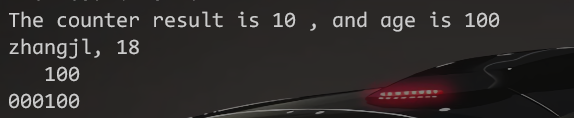
\includegraphics[width=\linewidth]{rust_format.png}
  \caption{格式化输出}
  \label{fig:rust_format}
\end{figure}
